% !TEX root = ../../../main.tex
% 来源：中学数学实验教材·第二册（几何）
% 章节：三角比与角边关系 / 锐角三角比
% 原始文件：6.tex，行 73-81
% 类型：tikz
% ---
    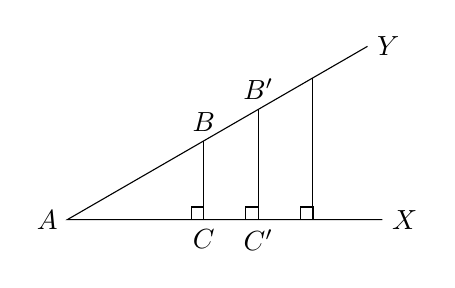
\begin{tikzpicture}[>=latex, scale=.8]
\draw(30:5.5)node[right]{$Y$}--(0,0)node[left]{$A$}--(5,0)node[right]{$X$};
\draw(30:2.5)node[above]{$B$}--+(0,-1.25)node[below]{$C$};
\draw(30:3.5)node[above]{$B'$}--+(0,-1.75)node[below]{$C'$};
\draw(30:4.5)--+(0,-2.25);
\draw(2.165,0) rectangle (2.165-.2,.2);
\draw(3.03,0) rectangle (3.03-.2,.2);
\draw(3.9,0) rectangle (3.9-.2,.2);
    \end{tikzpicture}
